\documentclass[12pt,oneside,openany,letterpaper]{article}


\usepackage{fancyhdr}
\usepackage{helvet}
\usepackage{amsmath}
%\usepackage{graphicx}
\usepackage{psfrag}
\usepackage{setspace}
%\usepackage[hypertex, linktocpage]{hyperref}[2003/11/30]
\usepackage[linktocpage]{hyperref}[2003/11/30]
\usepackage{lscape}
\usepackage{nicefrac}
\usepackage{mathrsfs}
\usepackage{units}
\usepackage{upgreek}
\usepackage{amssymb}
\usepackage{color}
\usepackage{wrapfig}
\usepackage{multirow}
\usepackage{url}
\usepackage{verbatim}
\usepackage[pdftex]{graphicx}
\usepackage{epstopdf}
\usepackage{enumitem}


\onehalfspacing \setlength\textheight{667pt}
\setlength\textwidth{506pt} \setlength\oddsidemargin{-18pt}
\setlength\topmargin{-20pt}
%\setlength\footskip{24pt}
\addtolength\headheight{2.5pt} \addtolength\headsep{-14pt}
%\fancyhead[R]{\includegraphics[height=10.5pt]{ubclogo_bw.eps}\#:  55907968}
%\renewcommand\familydefault{\sfdefault}


%\fancyhead[L]{Name:} \fancyhead[R]{Student
%Number:~~~~~~~~~~~~~~~~~~~~~~~~~~~~~~~~~~~~~~~~~~}
\fancyhead[L]{\emph{Introduction to Electronics}}\fancyhead[R]{All-Pass Filter}
\fancyfoot[L]{PHYS 231}\fancyfoot[R]{optional lab}
\pagestyle{fancy} \pagenumbering{arabic}




\begin{document}
\thispagestyle{plain}
\begin{center}
{\large{\bf{\fontfamily{phv}\selectfont Physics 231 - All-Pass Filter (Optional)}}}
\end{center}


\noindent In the lectures we looked at both low- and high-pass filters.  These circuits pass the input to the output unattenuated for a certain range of frequencies and attenuate the input at other frequencies.  There is also a frequency-dependent phase-shift of the output with respect to the input.  An ``all-pass'' filter is designed such that the ratio of the magnitudes of the input and output signals is equal to one for all frequencies (no attenuation), but the phase shift between the input and output is still frequency dependent.  These circuits can be used to delay a signal.

~

\noindent Figure~\ref{fig:active} shows one design for an all-phase filter. 
\begin{figure}[h!]
\begin{center}
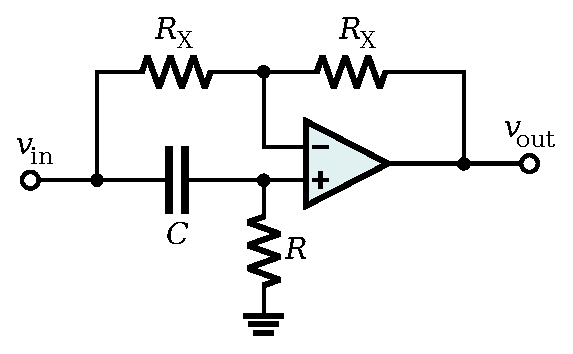
\includegraphics[width=7 cm]{figures/Active_Allpass_Filter.eps}
\caption{\label{fig:active} Active all-pass filter.}
\end{center}
\end{figure}
\newline Use the op-amp golden rules to show that:
\begin{equation}
\frac{v_\mathrm{out}}{v_\mathrm{in}}=\frac{j\omega R C-1}{j\omega R C+1}
\end{equation}
such that $\left\vert v_\mathrm{out}/v_\mathrm{in}\right\vert=1$ and:
\begin{equation}
\tan\phi=\frac{-2\omega RC}{1-\left(\omega RC\right)^2}.
\end{equation}
Take care when evaluating $\phi$ as $\tan\left(\pi/2+\delta\right)=\tan\left(-\pi/2+\delta\right)$.  This all-pass filter has zero phase shift at high frequency and a phase shift of $\pi$ at low frequency.  The phase shift between the input and output signals is $\pi/2$ when $\omega=(RC)^{-1}$.

~

\noindent The circuit in Fig.~\ref{fig:active} is an {\it active} all-pass filter because it uses an op-amp to provide gain to compensate for the losses that would occur in a usual $RC$ filter.  An all-pass filter using only {\it passive} components is shown in Fig.~\ref{fig:passive}.
\begin{figure}[h!]
\begin{center}
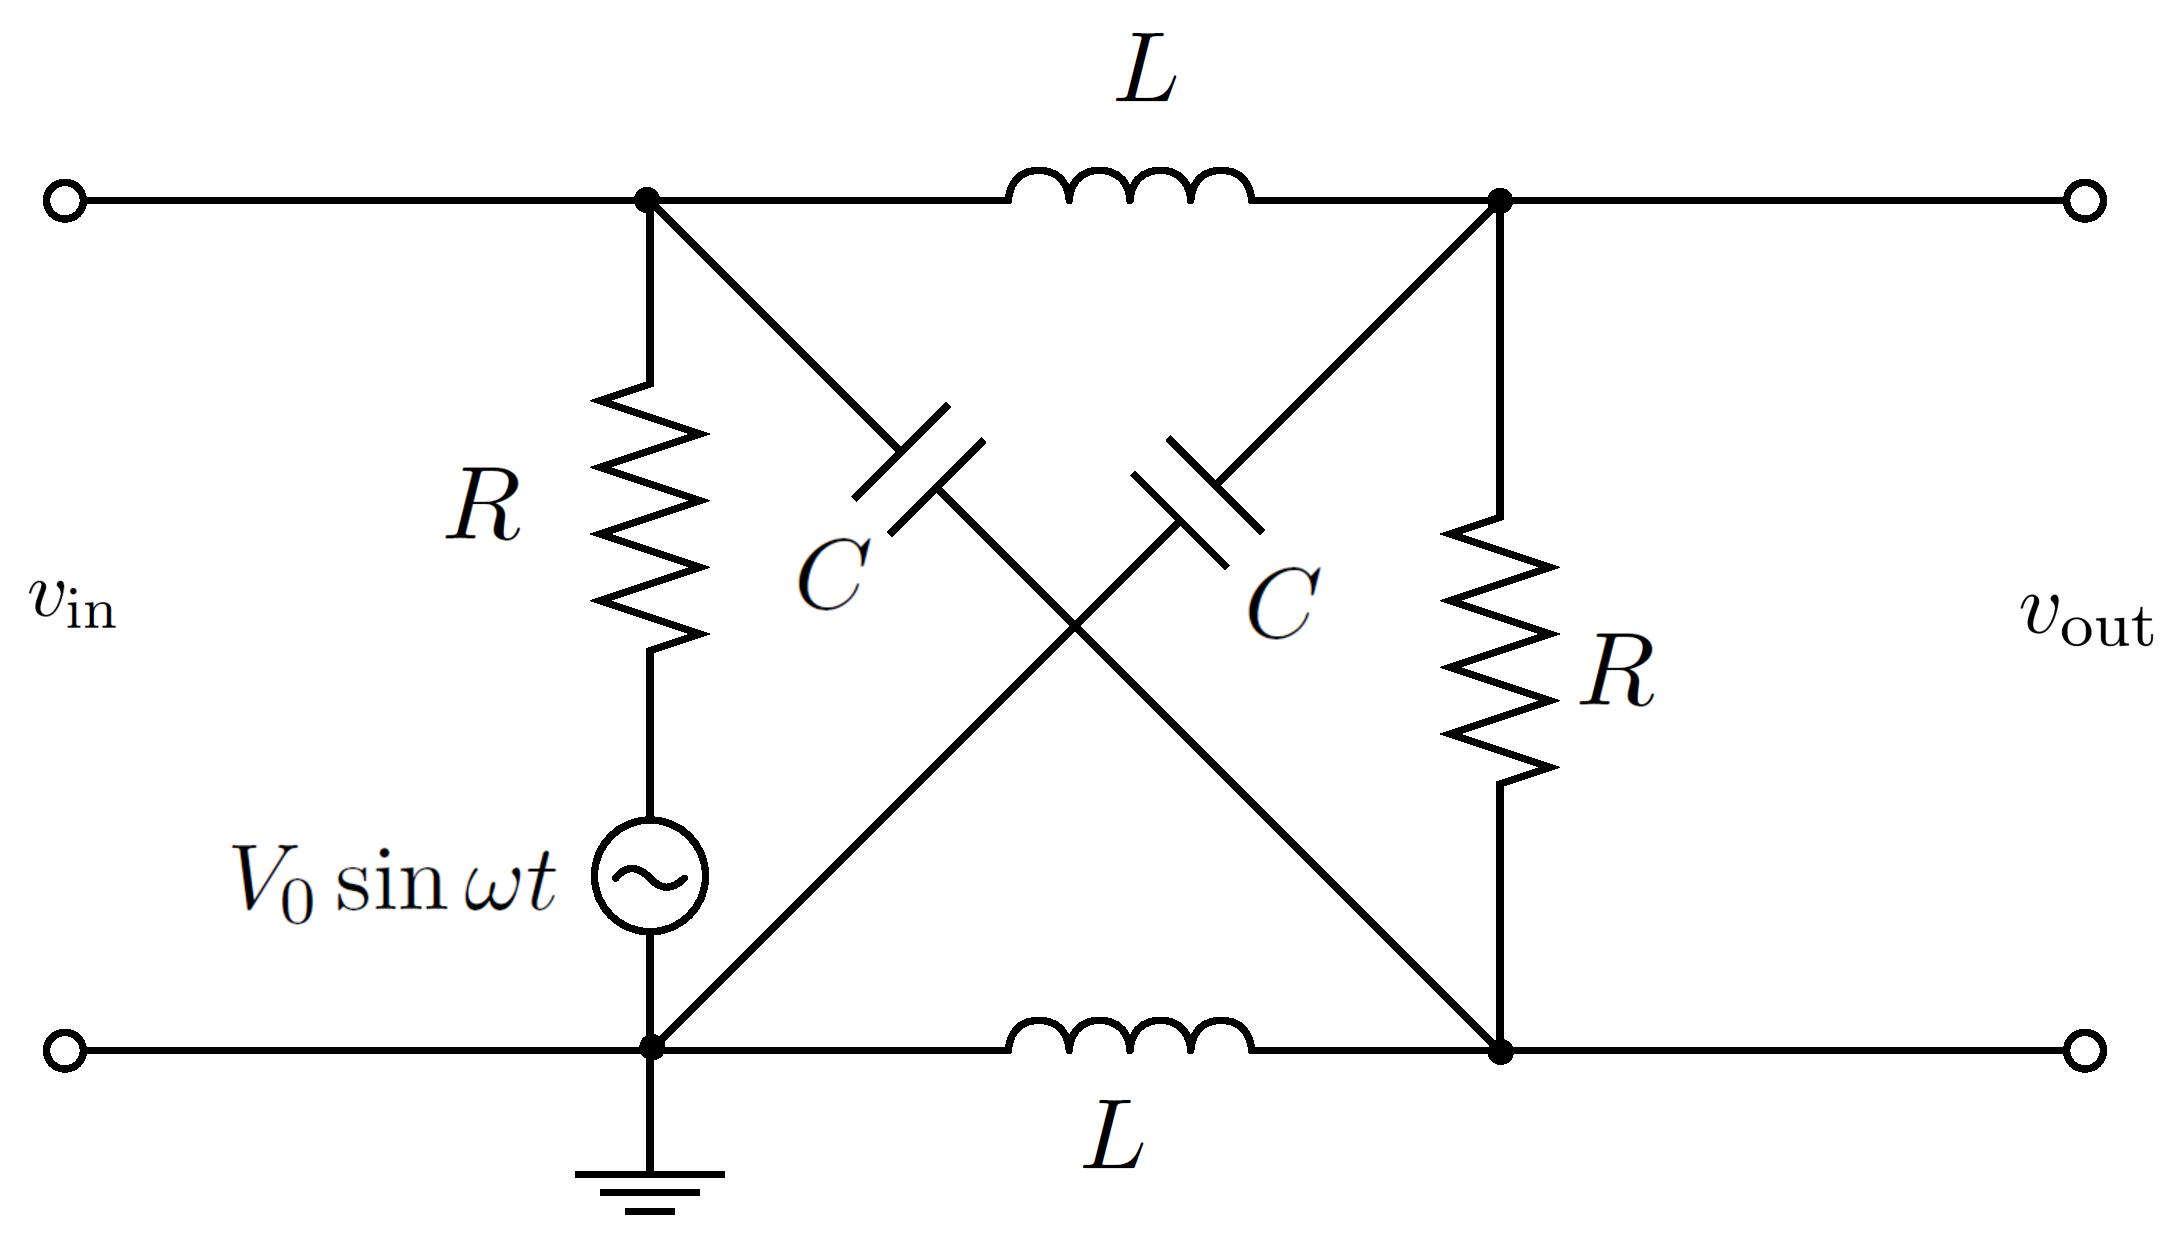
\includegraphics[width=10 cm]{figures/passiveAllPass.eps}
\caption{\label{fig:passive} Passive all-pass filter.}
\end{center}
\end{figure}

~

\noindent The passive circuit has the advantage that no external dc power supplies are required.  This circuit has six branches, all with different currents.  Determining $v_\mathrm{out}/v_\mathrm{in}$ requires that you solve a system of six equations with six unknowns.  Once the six equations have been determined, they are most easily solved using Maple.  Use Maple to show that:
\begin{equation}
\frac{v_\mathrm{out}}{v_\mathrm{in}}=\frac{1+\omega^2LC}{\left(1-\omega^2LC\right)+2j\omega\frac{L}{R}}.
\label{eq:pass}
\end{equation}
If the components are selected such that $R=\sqrt{L/C}$, then Eq.~\ref{eq:pass} can be rewritten as:
\begin{equation}
\frac{v_\mathrm{out}}{v_\mathrm{in}}=\frac{1+\omega^2\frac{L^2}{R^2}}{\left(1-\omega^2\frac{L^2}{R^2}\right)+2j\omega\frac{L}{R}}
\end{equation}
which is equivalent to:
\begin{equation}
\frac{v_\mathrm{out}}{v_\mathrm{in}}=\frac{1-j\omega\frac{L}{R}}{1+j\omega\frac{L}{R}}.
\label{eq:trans}
\end{equation}
Finally, Eq.~\ref{eq:trans} can be used to show that $\left\vert v_\mathrm{out}/v_\mathrm{in}\right\vert=1$ and:
\begin{equation}
\tan\phi=\frac{-2\omega\frac{L}{R}}{1-\omega^2\frac{L^2}{R^2}}.
\end{equation}
This all-pass filter has zero phase shift at low frequency, a phase shift of $-\pi$ at high frequency, and a phase shift of $-\pi/2$ when $\omega=R/L$.



\end{document}
